\documentclass[tikz, border=10pt]{standalone}
\usepackage{tikz}
\usetikzlibrary{positioning, shapes.multipart, arrows.meta}

\tikzset{
  topbox/.style={
    rectangle, rounded corners, draw=blue!50!black, fill=blue!15,
    thick, text centered, text width=4.5cm, minimum height=1.2cm, align=center
  },
  group/.style={
    rectangle, rounded corners, draw=blue!60!black, fill=blue!10,
    thick, text centered, minimum width=4.5cm, minimum height=1cm
  },
  project/.style={
    rectangle, draw=gray!50, fill=gray!10, thick,
    text width=6cm, minimum height=0.9cm, align=left
  },
  arrow/.style={thick, -{Stealth[round]}},
  root/.style={
    rectangle, draw=red!70, very thick, fill=red!10,
    text centered, minimum width=6cm, minimum height=1.2cm
  }
}

\begin{document}
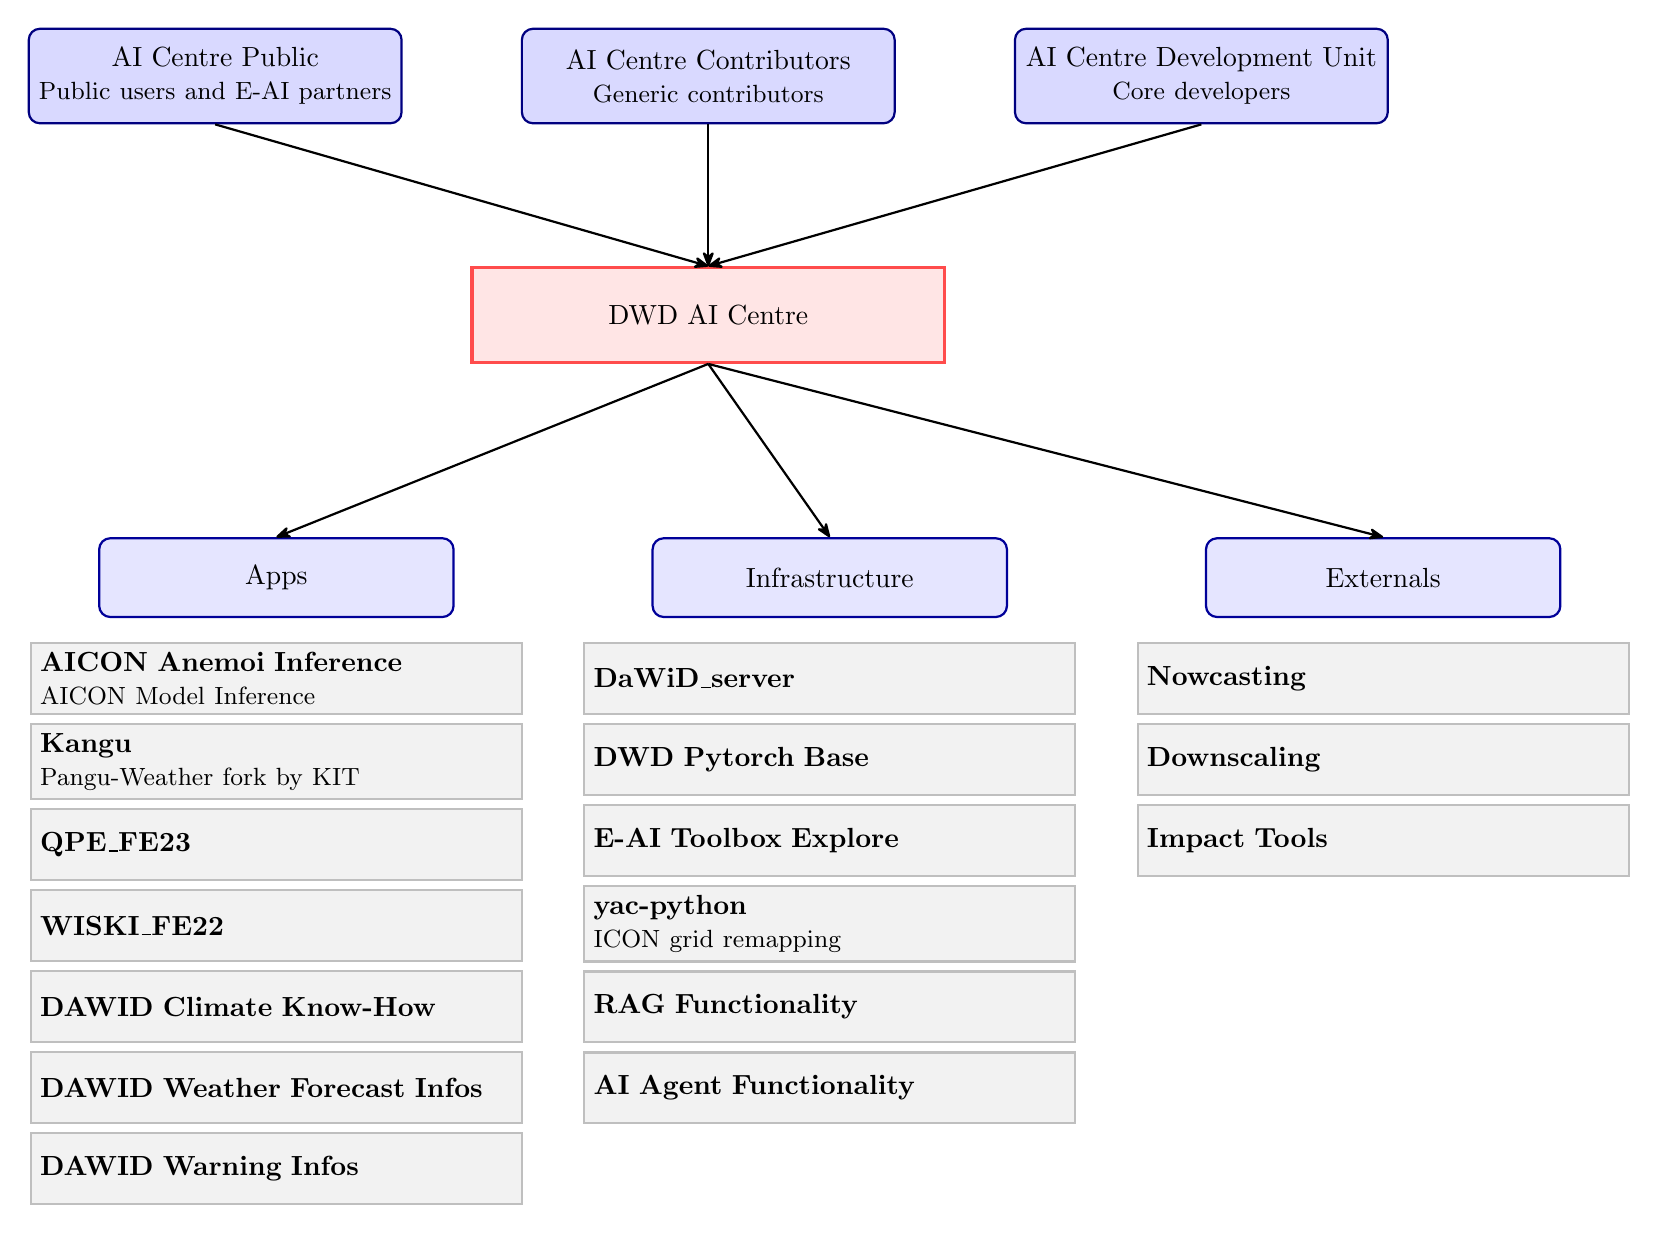
\begin{tikzpicture}[node distance=0.5cm]

% Top blue boxes
\node[topbox] (public) {AI Centre Public\\\small Public users and E-AI partners};
\node[topbox, right=1.5cm of public] (contributors) {AI Centre Contributors\\\small Generic contributors};
\node[topbox, right=1.5cm of contributors] (dev) {AI Centre Development Unit\\\small Core developers};

% Root node
\node[root, below=1.8cm of contributors] (root) {DWD AI Centre};

% Apps group
\node[group, below left=2.2cm and 0.2cm of root] (apps) {Apps};
\node[project, below=0.3cm of apps] (a1) {\textbf{AICON Anemoi Inference}\\ \small AICON Model Inference};
\node[project, below=0.1cm of a1] (a2) {\textbf{Kangu}\\ \small Pangu-Weather fork by KIT};
\node[project, below=0.1cm of a2] (a3) {\textbf{QPE\_FE23}};
\node[project, below=0.1cm of a3] (a4) {\textbf{WISKI\_FE22}};
\node[project, below=0.1cm of a4] (a5) {\textbf{DAWID Climate Know-How}};
\node[project, below=0.1cm of a5] (a6) {\textbf{DAWID Weather Forecast Infos}};
\node[project, below=0.1cm of a6] (a7) {\textbf{DAWID Warning Infos}};

% Infrastructure group
\node[group, right=2.5cm of apps] (infra) {Infrastructure};
\node[project, below=0.3cm of infra] (i1) {\textbf{DaWiD\_server}};
\node[project, below=0.1cm of i1] (i2) {\textbf{DWD Pytorch Base}};
\node[project, below=0.1cm of i2] (i3) {\textbf{E-AI Toolbox Explore}};
\node[project, below=0.1cm of i3] (i4) {\textbf{yac-python}\\ \small ICON grid remapping};
\node[project, below=0.1cm of i4] (i5) {\textbf{RAG Functionality}};
\node[project, below=0.1cm of i5] (i6) {\textbf{AI Agent Functionality}};

% Externals group
\node[group, right=2.5cm of infra] (ext) {Externals};
\node[project, below=0.3cm of ext] (e1) {\textbf{Nowcasting}};
\node[project, below=0.1cm of e1] (e2) {\textbf{Downscaling}};
\node[project, below=0.1cm of e2] (e3) {\textbf{Impact Tools}};

% Arrows from top to root
\draw[arrow] (public.south) -- (root.north);
\draw[arrow] (contributors.south) -- (root.north);
\draw[arrow] (dev.south) -- (root.north);

% Arrows to subgroups
\draw[arrow] (root.south) -- (apps.north);
\draw[arrow] (root.south) -- (infra.north);
\draw[arrow] (root.south) -- (ext.north);

\end{tikzpicture}
\end{document}
